\documentclass[aspectratio=169,12pt]{beamer}
\usepackage{fontspec}
\setsansfont{Inter}
\usepackage{booktabs}
\usepackage{graphicx}
\definecolor{ink}{HTML}{0B0B0B}
\definecolor{muted}{HTML}{52514E}
\definecolor{accent}{HTML}{1C5CAB}
\definecolor{paper}{HTML}{FCFCFB}
\setbeamercolor{background canvas}{bg=paper}
\setbeamercolor{normal text}{fg=ink}
\setbeamercolor{frametitle}{fg=ink}
\setbeamercolor{itemize item}{fg=accent}
\setbeamertemplate{navigation symbols}{}
\setbeamertemplate{itemize item}{\raisebox{0.15ex}{\small$\bullet$}}
\setbeamerfont{frametitle}{size=\Large,series=\bfseries}
\setbeamertemplate{frametitle}{\vspace{0.45cm}\insertframetitle}
\setbeamertemplate{footline}{\hfill{\tiny\color{muted}\insertframenumber\ / \inserttotalframenumber\hspace{0.6cm}}\vspace{0.3cm}}
\setbeamersize{text margin left=1.1cm,text margin right=1.1cm}
\setlength{\parskip}{6pt}
\newcommand{\bignum}[1]{{\fontsize{30}{34}\selectfont\bfseries\color{accent}#1}}
\newcommand{\sm}[1]{{\small\color{muted}#1}}
\newcommand{\N}{N}
\begin{document}

\begin{frame}[plain]
\vspace{1.0cm}
{\fontsize{30}{34}\selectfont\bfseries Do Their Numbers Match?}\\[0.45cm]
{\fontsize{13}{18}\selectfont Checking the figures in Nigerian national addresses\\ against the official releases they refer to}\\[0.75cm]
{\color{accent}\rule{1.6cm}{1.6pt}}\\[0.35cm]
{\fontsize{13}{16}\selectfont\bfseries Mia}\\[0.12cm]
{\fontsize{9}{12}\selectfont\color{muted}Apart Research AI × Epistemics Sprint \textbullet\ Track 4: Open Track}
\end{frame}

\begin{frame}{The question}
\vspace{0.3cm}
Political speeches lean on numbers. Each one comes from an official release, so each one can be checked.

For Nigeria, nobody has put the claims and the official figures side by side in a form others can audit.

\vspace{0.4cm}
{\Large\bfseries\color{accent}When Nigerian leaders quote a statistic,\\ does it match the official figure?}
\end{frame}

\begin{frame}{What was done}
\textbf{Five national addresses, chosen before any checking.}
\vspace{0.1cm}
\begin{itemize}\setlength{\itemsep}{7pt}
\item Four by the President, one by the main opposition candidate
\item \textbf{59} figures listed \textbullet\ \textbf{49} checked \textbullet\ \textbf{46} scored
\item Checked against the statistics bureau, central bank, budget office and others
\item Each row gets a verdict and a source link
\end{itemize}
\vspace{0.25cm}
\sm{Match: agrees. Close: within roughly 10 to 15 per cent. Mismatch: materially different,\\ or a different quantity from the one named.}
\end{frame}

\begin{frame}{Result: four in five matched}
\vspace{0.1cm}
\begin{columns}[T]
\begin{column}{0.30\textwidth}
\bignum{37}\ \ match\\[0.25cm]
\bignum{5}\ \ close\\[0.25cm]
\bignum{4}\ \ mismatch
\end{column}
\begin{column}{0.68\textwidth}
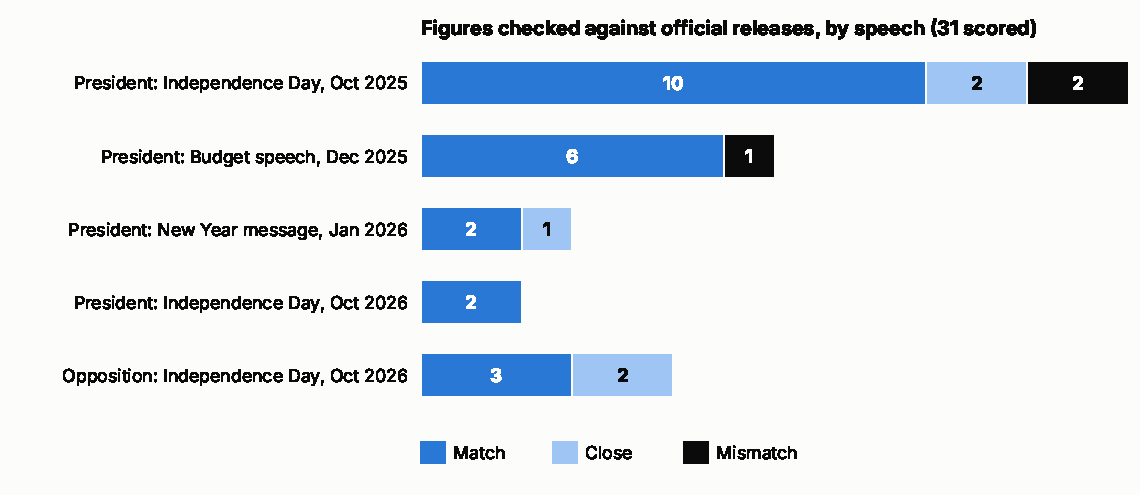
\includegraphics[width=\linewidth]{figure1.pdf}
\end{column}
\end{columns}
\vspace{0.3cm}
\sm{Every specific growth and inflation rate quoted in the five speeches matched exactly.}
\end{frame}

\begin{frame}{Biggest misses: ``non-oil'' with oil in it}
\vspace{0.2cm}
\textbf{Claim:} non-oil exports are now 48\% of exports.
\vspace{0.3cm}

\begin{tabular}{lr}
\toprule
Official trade release, Q2 2025 & Share of exports \\
\midrule
Crude oil & 52.60\% \\
Other petroleum products and gas & 34.21\% \\
\textbf{Non-oil products} & \textbf{13.39\%} \\
\bottomrule
\end{tabular}
\vspace{0.35cm}

\sm{The 48\% is everything except \emph{crude}.}

\textbf{Same speech:} non-oil revenue of ``over \N 20 trillion'' by August.\\ That was \emph{total} revenue. Non-oil was \textbf{\N 15.7 trillion}.
\end{frame}

\begin{frame}{How the other figures went wrong}
\begin{itemize}\setlength{\itemsep}{8pt}
\item \textbf{Out of date:} a stock market gain quoted from ten days earlier
\item \textbf{Wrong baseline:} oil output ``from barely one million'' in May 2023. It was 1.18 million; the lower figure was April
\item \textbf{Both directions:} of eight errors with a direction, five helped the speaker and three hurt
\end{itemize}
\vspace{0.2cm}
\textbf{Two claims fit no verdict.} Two official sources give different foreign investment figures. One debt ratio has no published source at all.
\end{frame}

\begin{frame}{Can you trust the verdicts?}
\textbf{Two independent checks.}
\vspace{0.1cm}
\begin{itemize}\setlength{\itemsep}{8pt}
\item \textbf{A script with no AI in it} found every recorded number in its source for 39 of 46 rows, and the quoted figures in six more
\item \textbf{A blind second coder}, a different AI model, gave the same verdict on 32 of 45
\end{itemize}
\vspace{0.2cm}
\bignum{80\%}\ \ vs\ \ \bignum{73\%}\ \ \sm{match rate, first and second checker}

\sm{Most figures match under either checker. Single verdicts near the boundaries are less reliable, and the second coder disputed the revenue finding.}
\end{frame}

\begin{frame}{What it is, and what it is not}
\begin{itemize}\setlength{\itemsep}{8pt}
\item An open dataset with a source link on every scored row
\item A small test set for claim-checking tools in a setting they rarely see
\item \textbf{Small:} 46 scored figures, 10 still unchecked
\item \textbf{No human checker}, and mostly press reports of official releases
\item Not a comparison of the two speakers, and not a fact-check of record
\end{itemize}
\vspace{0.3cm}
{\bfseries\color{accent}github.com/Mhiah/Tally}
\end{frame}

\end{document}
